\documentclass[11pt]{beamer}
\usetheme{Goettingen}
\usepackage[utf8]{inputenc}
\usepackage{amsmath}
\usepackage{amsfonts}
\usepackage{amssymb}
\usepackage{graphicx}
\usepackage{cite}
\usepackage{hyperref}
\author{Habib Balit}
\title{Vision Par Ordinateur}
\institute{Université Paris 8}
\date{Jeudi 6 Mai 2019}
%\setbeamercovered{transparent} 
%\setbeamertemplate{navigation symbols}{} 
%\logo{} 
%\institute{} 
%\date{} 
%\subject{} 
\begin{document}

\begin{frame}
\titlepage
\end{frame}


\begin{frame}
\tableofcontents
\end{frame}

\section{Introduction}
\begin{frame}
\frametitle{Introduction}
\begin{center}
	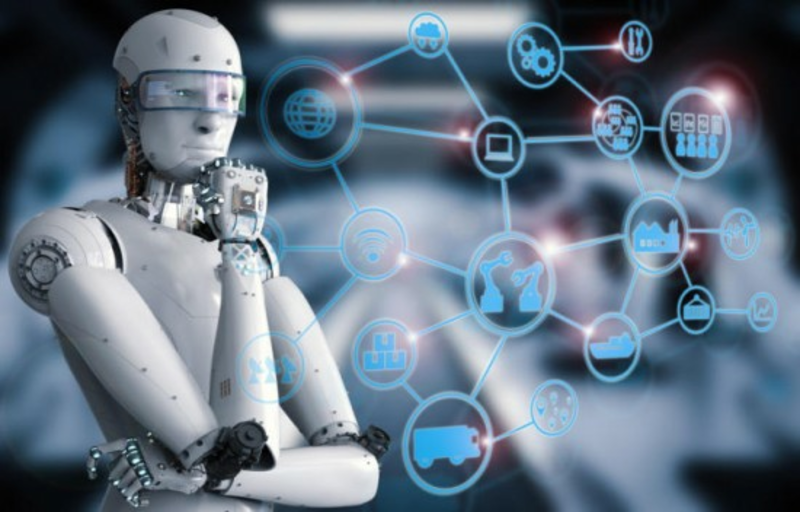
\includegraphics[scale=0.2]{img2.png}
\end{center}
Une science qui a pour objectifs de traiter et transformer les images et vidéos prises par la machine.
\end{frame}

\section{Application}
\begin{frame}
\frametitle{Application}
\begin{minipage}{0.4\textwidth}
	\begin{flushright}
		\begin{itemize}
		\item La santé.
		\item Les automobiles.
		\item La surveillance.
		\item L'astronomie.
		\item L'agriculture.
		\item L'industriel.
		\item L'imagerie par satellites.
		\end{itemize}
	\end{flushright}
\end{minipage}
\begin{center}
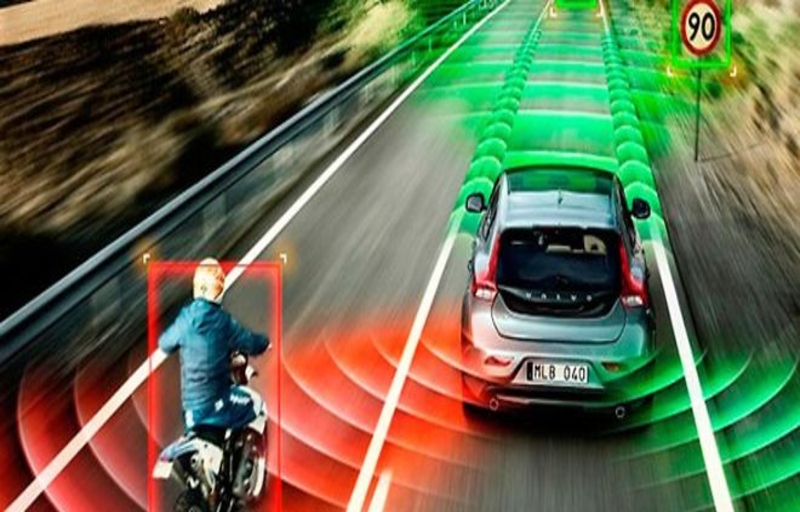
\includegraphics[scale=0.1]{img4.png}
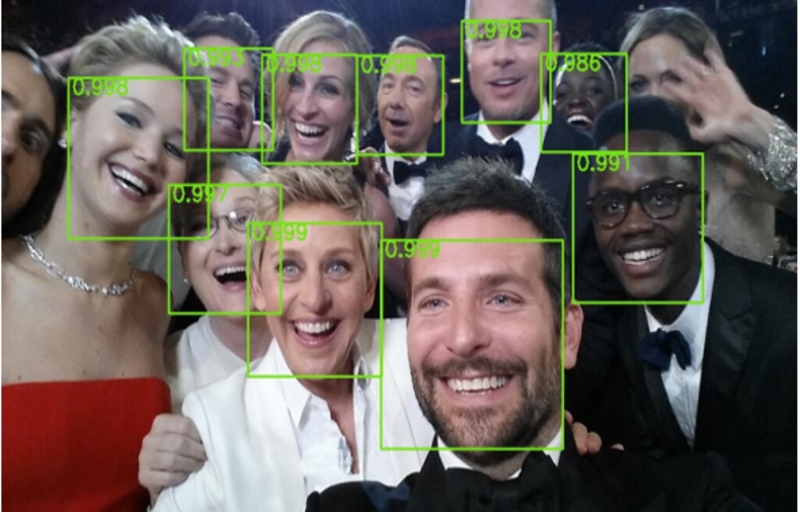
\includegraphics[scale=0.1]{img5.png}
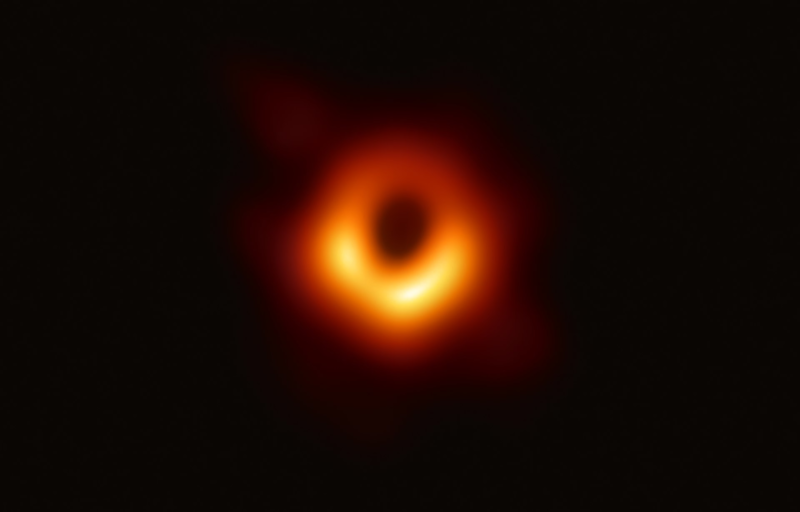
\includegraphics[scale=0.1]{img6.png}
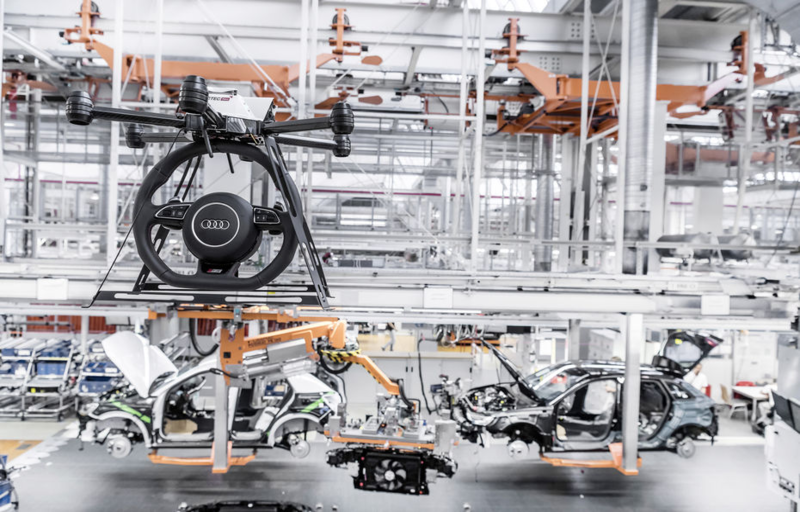
\includegraphics[scale=0.1]{img7.png}
\end{center}
\end{frame}

\section{CNN}
\subsection{Définition}
\begin{frame}
\frametitle{Définition}
\begin{itemize}
\item Un réseau multicouches, inspirer du néocognitron.
\begin{center}
	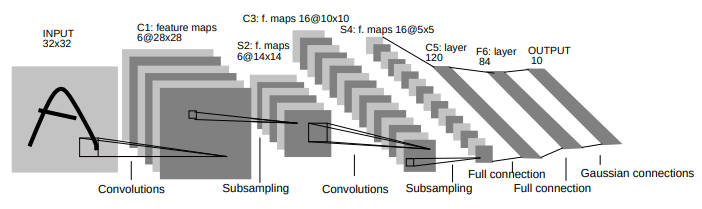
\includegraphics[scale=0.35]{img25.png}
\end{center}
\item conçus pour reconnaître des formes à partir d’images.
\item reconnaissance des modèles extrêmement variés. 
\item robustes aux distorsions et aux transformations géométriques.
\end{itemize}
\end{frame}

\subsection{Les couches d'un CNN}
\begin{frame}
\frametitle{Les couches de bases d'un CNN}
\begin{itemize}
	\item Convolution 
	\item Max Pooling
	\item Flattening
	\item Fully Connected
\end{itemize}
\end{frame}

\subsubsection{Convolution}
\begin{frame}
\frametitle{Convolution}

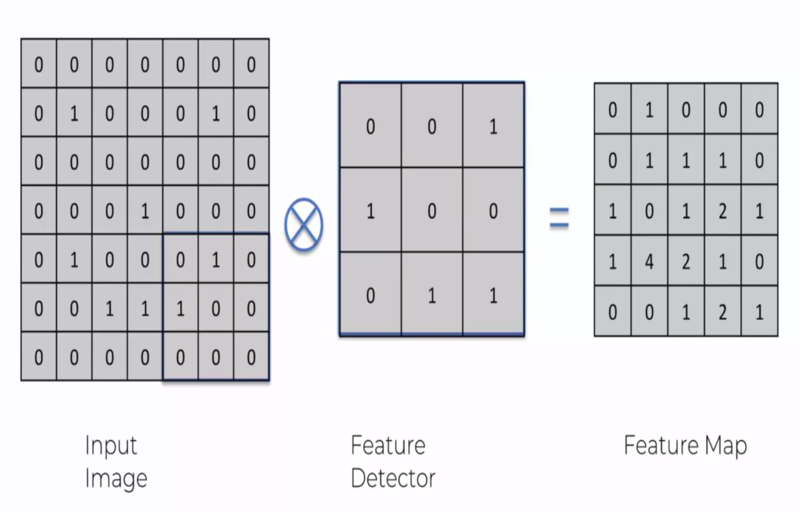
\includegraphics[scale=0.17]{img10.png}
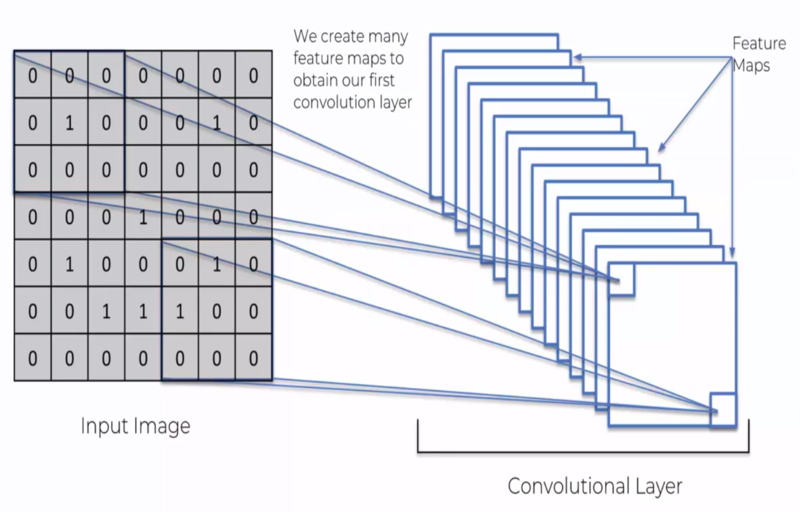
\includegraphics[scale=0.17]{img11.png}

Afin d'éviter la linéarité, on applique une fonction $\phi = max(x, 0)$.
\end{frame}
\subsubsection{Max Pooling}
\begin{frame}
\frametitle{Max Pooling}
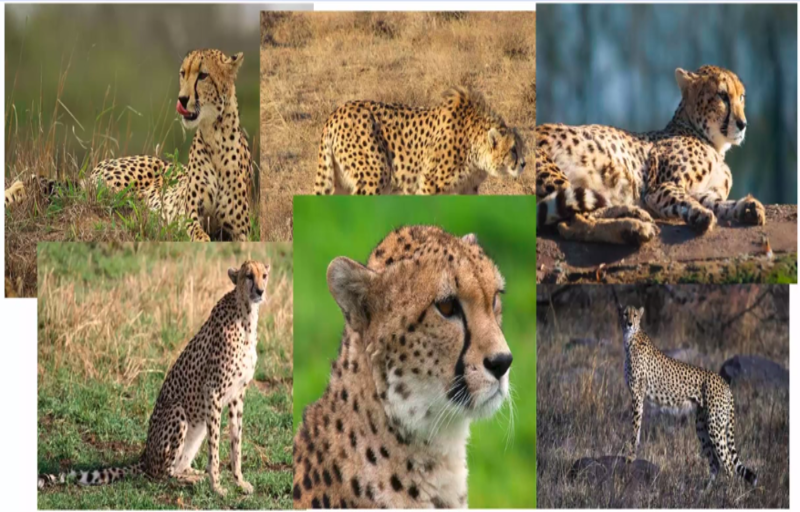
\includegraphics[scale=0.17]{img14.png}
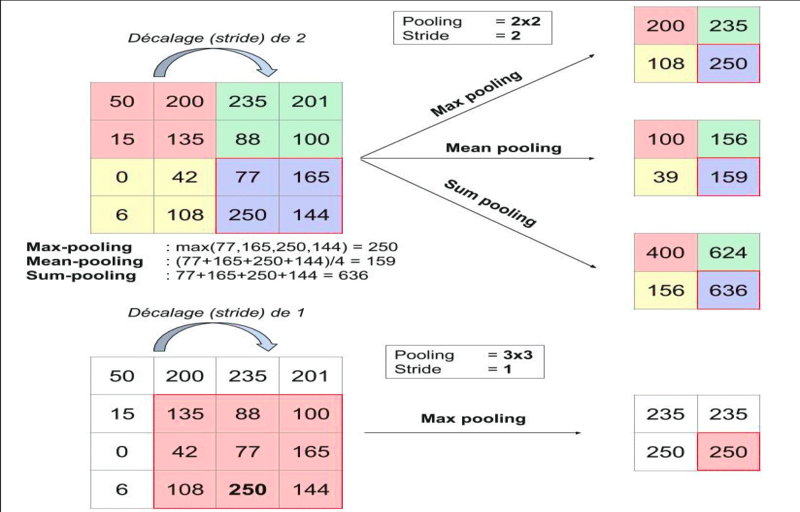
\includegraphics[scale=0.17]{img15.png}

La propriété de l'invariance spatiale:
\begin{itemize}
	\item Max Pooling
	\item Mean Pooling
	\item Sum Pooling
\end{itemize}
\end{frame}
\subsubsection{Flattening}
\begin{frame}
\frametitle{Flattening}
\begin{center}
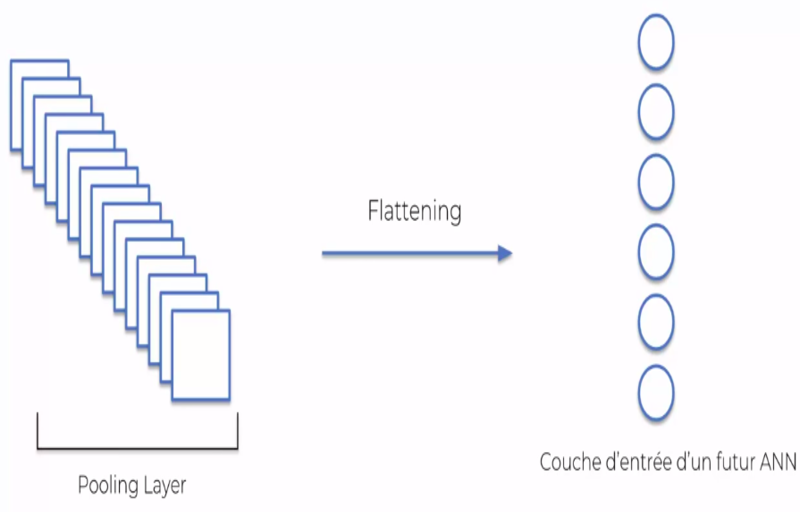
\includegraphics[scale=0.25]{img16.png}
\end{center}

création d'un grand vecteur qui sert comme une couche d’entrée au futur réseau de neurone.
\end{frame}
\subsubsection{Fully Connected}
\begin{frame}
\frametitle{Fully Connected}
\begin{center}
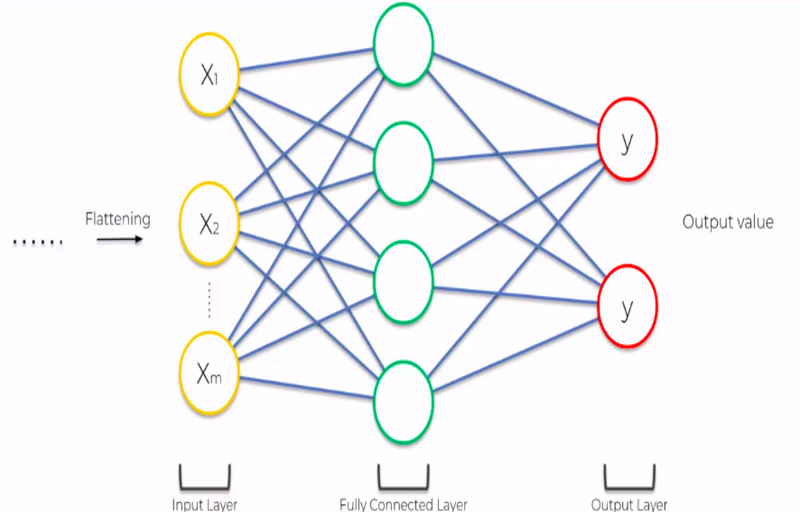
\includegraphics[scale=0.17]{img17.png}
\end{center}
Un perceptron multicouches, qu'est constitué :
\begin{itemize}
	\item des neurones d’entrés
	\item des neurones cachés :\\ ($\phi (\sum_{i=0}^{m} w_{i} x_{i})$ ou  $\phi$ est une fonction d’activation.)
	\item des neurones de sortie
\end{itemize}
\end{frame}








\subsection{Architectures CNN}
\begin{frame}
\frametitle{Architectures CNN}
\begin{center}
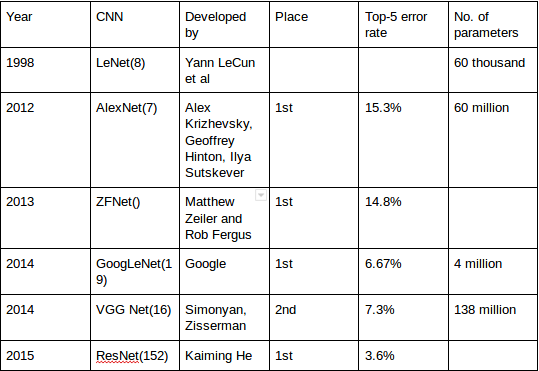
\includegraphics[scale=0.4]{img32.png}
\end{center}
ImageNet Large Scale Visual Recognition Challenge (ILSVRC).
\end{frame}
\begin{frame}
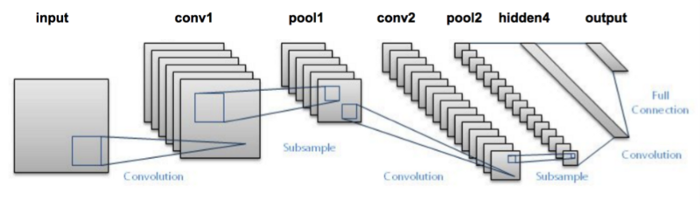
\includegraphics[scale=0.19]{img27.png}
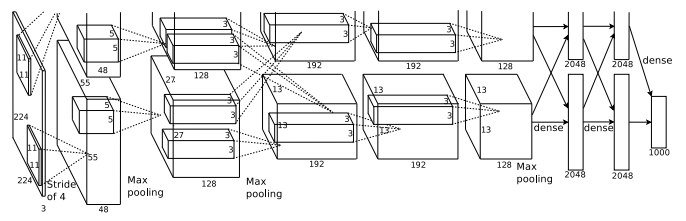
\includegraphics[scale=0.19]{img28.png}
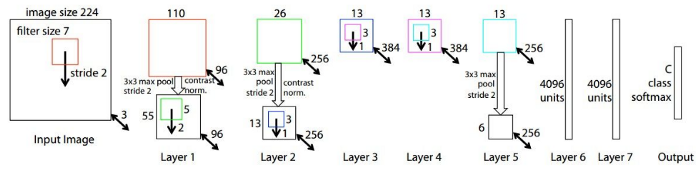
\includegraphics[scale=0.19]{img29.png}
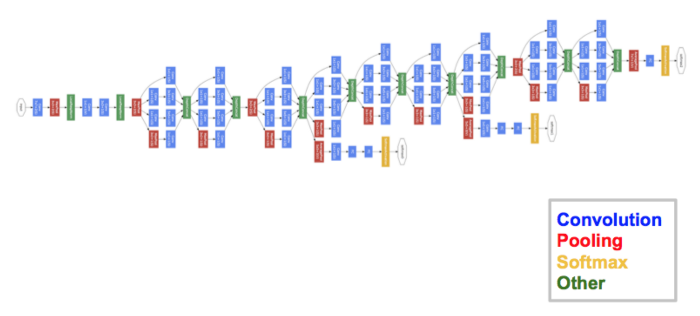
\includegraphics[scale=0.19]{img30.png}
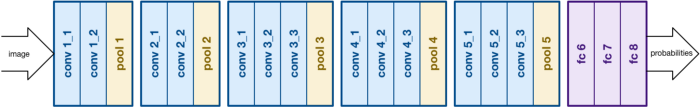
\includegraphics[scale=0.19]{img31.png}
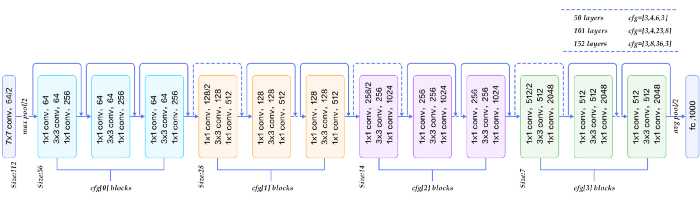
\includegraphics[scale=0.19]{img26.png}
\\
\begin{center}
Sources : \href{https://medium.com/@sidereal/cnns-architectures-lenet-alexnet-vgg-googlenet-resnet-and-more-666091488df5}{https://medium.com/@sidereal/}
\end{center}
\end{frame}

\section{Conclusion}
\begin{frame}
\frametitle{Conclusion}
\begin{itemize}
	\item La partie théorique.
	\item Les réseaux utilisés par la communauté
	\item implémentation ?
	\item \cite{fukushima1980neocognitron},
\cite{lecun1995convolutional},
\cite{lecun1998gradient},
\cite{scherer2010evaluation} et 
\cite{wu2017convolutional}
	\item Les images sont prises d'un cours en ligne sur udemy " le deep learning de a à z ".
\end{itemize}
\end{frame}

\begin{frame}
\bibliographystyle{unsrt}
\bibliography{b} 
\end{frame}


\begin{frame}
\begin{center}
\textbf{\Large{Merci pour votre attention}}
\end{center}
\end{frame}

\end{document}